 \documentclass{beamer}
 
 \usepackage{amsmath}
 \usepackage{graphics}
 \usepackage{graphicx}
 \usepackage{framed}
 \usepackage{amssymb}
 
 \begin{document}
%===

% % SLIDE 1 - COVER SLIDE
\begin{figure}
\centering

\includegraphics[width=0.9\linewidth]{Rlogo}
\end{figure}
\[ \mbox{Introduction to R} \] 


%===

{Introduction to R}
Source: R project website (http://www.r-project.org)

* R is a language and environment for statistical computing and graphics. It is a GNU project
which is similar to the S language and environment which was developed at Bell Laboratories
(formerly AT\&T, now Lucent Technologies) by John Chambers and colleagues. 
* R can be considered
as a different implementation of S. There are some important differences, but much
code written for S runs unaltered under R.




%===

{What is R?}

* R provides a wide variety of statistical (linear and nonlinear modelling, classical statistical tests,
time-series analysis, classification, clustering, ...) and graphical techniques, and is highly extensible.
* The S language is often the vehicle of choice for research in statistical methodology,
and ``R} provides an Open Source route to participation in that activity.
* One of ``R}’s strengths is the ease with which well-designed publication-quality plots can be
produced, including mathematical symbols and formulae where needed. 




%===

{What is R?}

* Great care has been
taken over the defaults for the minor design choices in graphics, but the user retains full control.
* ``R} is available as Free Software under the terms of the Free Software Foundation’s GNU General
Public License in source code form. It compiles and runs on a wide variety of UNIX platforms
and similar systems (including FreeBSD and Linux), Windows and MacOS.


%===


{What is R?}
``R} is a programming environment that

* uses a well-developed but simple programming language
* allows for rapid development of new tools according to user demand
* these tools are distributed as packages, which any user can download to customize the R
environment.


%===

% % SLIDE 1 - COVER SLIDE
\begin{figure}
\centering
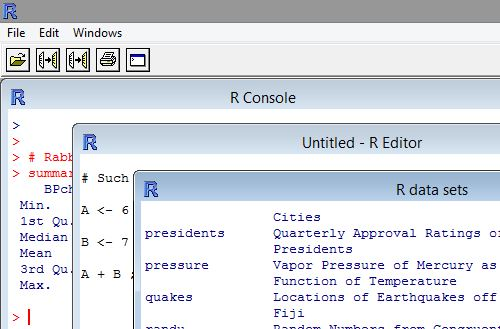
\includegraphics[width=1.2\linewidth]{images/Rmultiplewindows}
\end{figure}

   

%===

{Comprehensive R Archive Network}

* Base ``R} and most ``R} packages are available for download from the \textbf{Comprehensive R Archive Network}
(CRAN) cran.r-project.org. 
* Base ``R} comes with a number of basic data management,
analysis, and graphical tools 
* ``R}s power and flexibility, however, lie in its array of packages
(currently more than 6,000!)



%========== %
 
\begin{figure}
\centering
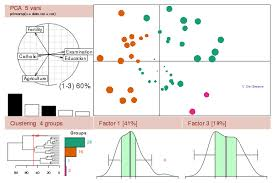
\includegraphics[width=1.2\linewidth]{CRAN}
\end{figure}

% %

{Introduction to R}
\textbf{Secton 1 - A few basics} 

\item[1.1] Installing ``R}      
\item[1.2] Command Line Interface     
\item[1.3] The Assignment operator     
\item[1.4] Commenting      
\item[1.5] Defining Variables     
\item[1.6] Help Functions      
\item[1.7] The ``help.start()`` command     
\item[1.8] Basic Maths Operations     
\item[1.9] Basic ``R} Editor      


%===

{1.1 Installing R}

* ``R} is very easily installed by downloading it from the CRAN website. Installation usually takes
about 2 minutes. 
* When installation of R is complete, the distinctive ``R} icon will appear on your
desktop. To start ``R}, simply click this Icon. 
* It is common to re-install ``R} once a year or so. The
current version of ``R}, version 3.1.2 was released quite recently.





%===

% % SLIDE 1 - COVER SLIDE
\begin{figure}
\centering
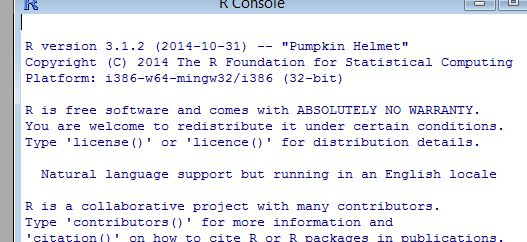
\includegraphics[width=1.2\linewidth]{images/Rversion}        
\end{figure}
  
%===


{1.2 Command Line Interface}

* When you start ``R}, the command line interface window will appear on screen. This is one
of many windows in the ``R} environment, others including graphical output windows, or script
editors. 
* ``R} code can be entered into the command line directly. 
* Alternatively code can be saved
to a script, which can be run inside a session using the ``source()`` function.


%===

{1.3 The Assignment operator}

* The assignment operator is used to assign names to particular values. 
* Historically the assignment
operator was ) a ````$<-$}”. 
* The assignment operator can also be the equals sign "=". (This is valid as of ``R}
version 1.4.0.)

* Both will be used, although, you should learn one and stick with it. Many long term ``R}
users prefer the arrow approach. 



%===

{1.3 The Assignment operator}

* You can also use $->$ as an assignment operator, reversing the
usual assignment positions. (This is actually really useful).
* Commands are separated either by
a semi colon or by a newline.

\begin{figure}
\centering
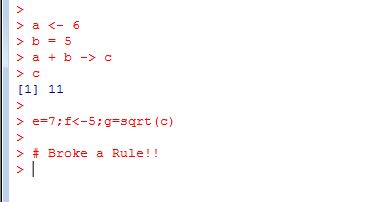
\includegraphics[width=1.2\linewidth]{images/assignment}
%\caption{}
%\label{fig:assignment}
\end{figure}



%===

{1.3 The Assignment operator}
\textbf{The Up and Down Keys}

* Before we continue, try using the up and down keys, and see what happens. 
* Previously
typed commands are re-presented, and can be re-executed.



%===

{1.3 The Assignment operator }
\textbf{objects}

* R stores both data and output from data analysis (as well as everything else) in \textbf{objects}.
* The variables we have created so far are objects. 
* A list of all objects in the current session can
be obtained with ``ls()``.


\textbf{1.3.1 Reserved Words - Bad names for Objects}

* Some names are used by the system, e.g.``T, F,q,c} etc . 
* Avoid using these. (This is the rule I broke earlier on)
* Also avoid using command names like \textbf{mean} and \textbf{sum}



  
%===

{1.4 Commenting}
For the sake of readability, it is good practice to comment code. The \# character at the
beginning of a line signifies a comment, which is not executed. Lines of hashtags can be used
to identify the beginning and end of code segments
\begin{figure}
\centering
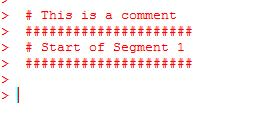
\includegraphics[width=1.2\linewidth]{images/commenting}
%\caption{}
%\label{fig:commenting}
\end{figure}


%===

{1.5 Defining and Naming Variables}

* A convention is to use define a variable name with a capital letter (R is case sensitive). 
* This
reduces the chance of overwriting in-build ``R} functions, which are usually written in lowercase
letters. 
* Commonly used variable names such as x, y and z (in lower case letters) are not “reserved”.

\textbf{Camel Case}
\begin{framed}
``camelCase}

``variableName}

``AlsoCamelCase}
\end{framed}


%===


{1.6 Help Functions}

*  Help files for R functions are accessed by preceding the name of the function with ?\\  (e.g. ``?sort}
). 

* Alternatively you can use the command ``help()`` (e.g. ``help(sqrt)} )



%===


{1.6 Help Functions}

* A HTML document appears on screen with information on the function typed in. 
* As well
as the list of arguments that the particular function accepts, and how to specify them, there is
example code at the bottom of the file. 
* These code segments are often invaluable in learning
how to master the function.





%===

% % SLIDE 1 - COVER SLIDE
\begin{figure}
\centering
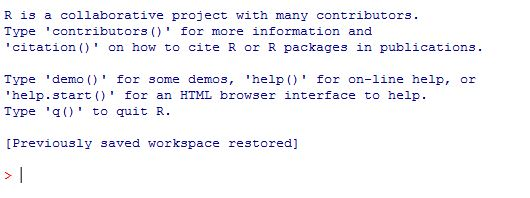
\includegraphics[width=1.2\linewidth]{images/Rhelpcommands}
%%\caption{}
%%\label{fig:Rhelpcommands}
\end{figure}
   


 
%===



{1.7 The ``help.start()`` command}
As mentioned by the text on the main console, the ``help.start()`` command can be usd to
access detailed help documentation that comes as part of the installation.


\begin{figure}
\centering
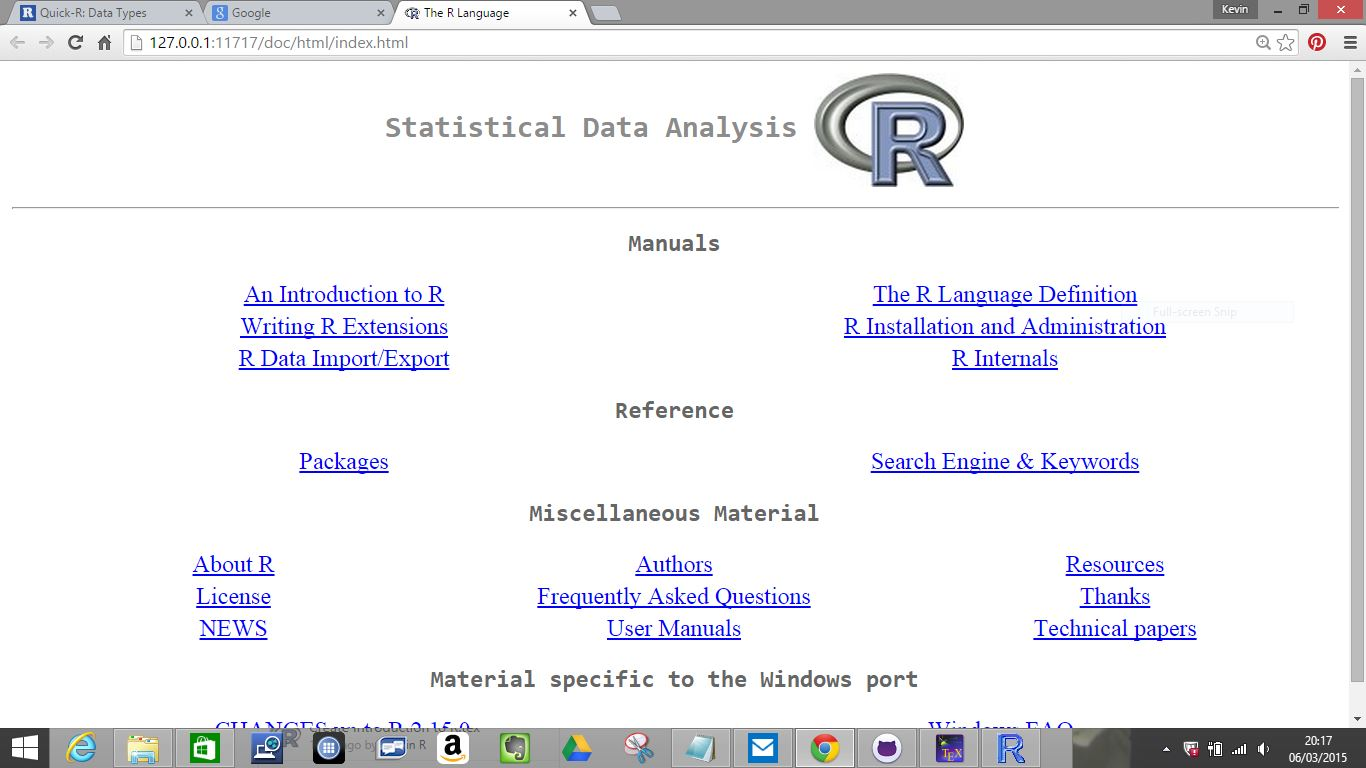
\includegraphics[width=1.2\linewidth]{images/helpstart}

\end{figure}

%===


{1.8 Basic Maths Operations}
\vspace{-0.5cm}
The most commonly used mathematical operators are all supported by ``R}. \\  Here are a few
examples:
\begin{tabular}{|c|c|} \hline
$5 + 3 \ast 5$ &  Note the order of operations.\\\hline
log (10) & Natural logarithm with base e=2.718282 \\\hline
log(8,2) & Log to the base 2 \\\hline
$4^2$ & 4 raised to the second power \\\hline
7/2 & Division \\\hline
factorial(4) & Factorial of Four \\\hline
sqrt (25) & Square root \\\hline
abs (3-7) & Absolute value of 3-7 \\\hline
pi & The mysterious number \\\hline
exp(2) & exponential function \\\hline

\end{tabular} 


%===


``R} can be used for many mathematical operations, including


* Set Theory
* Trigonometry
* Complex Numbers
* Binomial Coefficients

Set Theory is always useful to know (Monty Hall Problem). We will not go into any of the others in great detail today.


%===

{1.9 Basic ``R} Editor}

* ``R} has an inbuilt script editor. We will use it for this class, but there are plenty of top quality
Integrated Development Environments out there. (Read up about \textbf{RStudio} for example).
* For a while, we will use the in-built script editor. Although it is advisable to start using \textbf{Rstudio} or something similar in the not-too-distant future.




%===

% % SLIDE 1 - COVER SLIDE
\begin{figure}
\centering
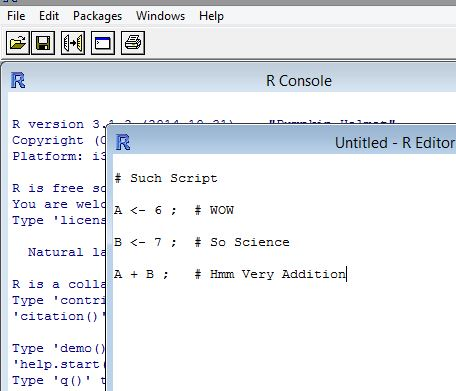
\includegraphics[width=1.2\linewidth]{images/Rscript}         
\end{figure}
   
%===

{1.9 Basic ``R} Editor}

* To start a new script, or open an existing script simply go to File and click the appropriate
options. A new dialogue box will appear. 

* You can write and edit code using this editor.
* To pass the code for compiling , press the run line or selection option (The third icon
on the menu).


%===



* Another way to read code is to use the ``edit()`` function, which operates directly from the
command line. 
* To see how the code defining an object X was written (or more importantly,
could have been written) simply type ``edit(X)}. 
* This command has some useful applications
that we will see later on (the ``scan()`` command).



%===


\textbf{Script Files}

* Scripts are saved as ``.R} files. 
* These scripts can be called directly using the ``source()`` command.


\begin{framed}
``source(myScript.R)}

``source(myDatasets.R)}

``source(myFunctions.R)}
\end{framed}


% %

{Introduction to R - Continued}

\item[1.10] Built-In Data Sets      
\item[1.11] The ``summary()`` command     
\item[1.12] Working directories      
\item[1.13] Coming Unstuck    
\item[1.14] Quitting the ``R} environment   
\item[1.15] Data Objects  
\item[1.16] Listing all items in a workspace     
\item[1.17] Removing items   
\item[1.18] Checking and Transforming Types
\item[1.19] Saving and Loading R Data Objects    




%===

{1.10 Built-In Data Sets}
\textbf{Inbuilt Data Sets}\\
Several data sets , intended as learning tools, are automatically installed when R is installed.
Many more are installed within packages to complement learning to use those packages. \\


\textbf{iris}\\ One
of these is the famous Iris data set, which is used in many data mining exercises.


* airquality  ( very useful )
* mtcars
* Nile

More are available once packages are loaded.


%===

% % SLIDE 1 - COVER SLIDE
\begin{figure}
\centering
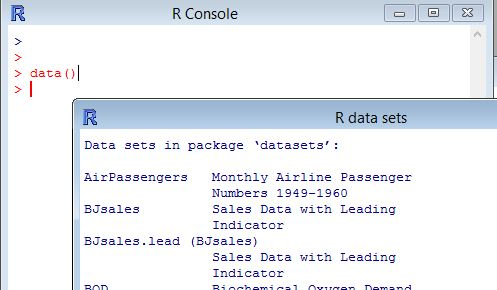
\includegraphics[width=1.2\linewidth]{images/Rdatasets}        
\end{figure}
   
%===

% % SLIDE 1 - COVER SLIDE
\begin{figure}
\centering
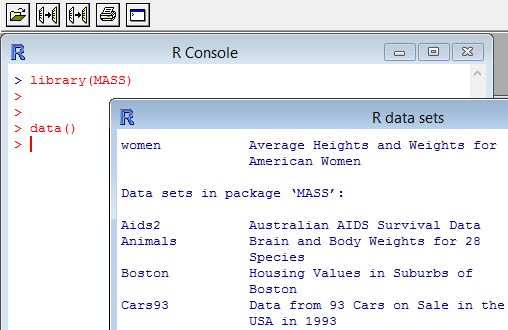
\includegraphics[width=1.2\linewidth]{images/RdatasetsMore}   
\end{figure}
   
%===



* To see what data sets are available, simply type ``data()``.
*  To load a data set, simply type in the
name of the data set. Some data sets are very large.
*  To just see the first few (or last) rows, we
use the ``head()`` function or alternatively the ``tail()`` function. 
* The default number of rows of
these commands is 6. Other numbers can be specified.



%===

% % SLIDE 1 - COVER SLIDE
\begin{figure}
\centering 
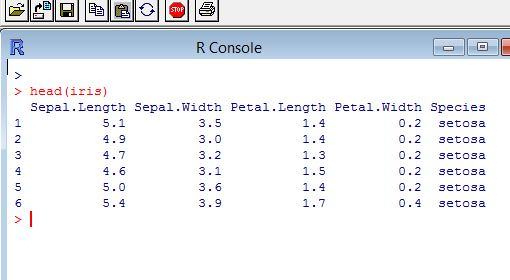
\includegraphics[width=1.2\linewidth]{images/irishead}      
\end{figure}
   
%===

% % SLIDE 1 - COVER SLIDE
\begin{figure}
\centering
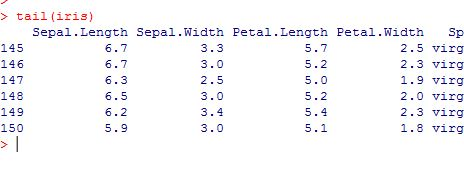
\includegraphics[width=1.2\linewidth]{images/iristail}     
\end{figure}
   
%===


* In many situations, it is useful to call a particular data set using the ``attach()`` command. This
will save having to specify the data sets over repeated operations. 
* The file can then be detached
using the ``detach()`` command.





%===

{1.11 The summary() command}


* The R command ``summary()`` is a generic function used to produce result “summaries” of the
results of various objects, from simple vectors to the output of complex model fitting functions.
* The function invokes particular methods which depend on the class of the first argument.


%===

% % SLIDE 1 - COVER SLIDE
\begin{figure}
\centering
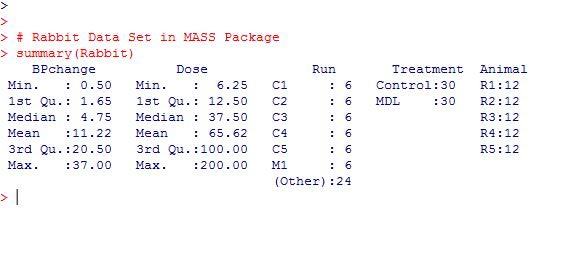
\includegraphics[width=1.2\linewidth]{images/rabbitsummary}   
\end{figure}
 

%===

% % SLIDE 1 - COVER SLIDE
\begin{figure}  
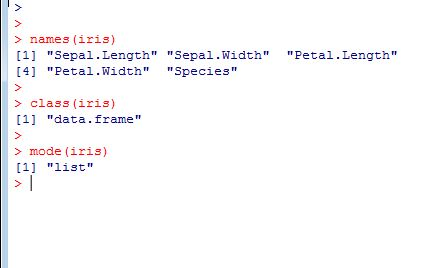
\includegraphics[width=1.2\linewidth]{images/irisinspect}     
\end{figure}
   
%===

% % SLIDE 1 - COVER SLIDE
\begin{figure}
\centering
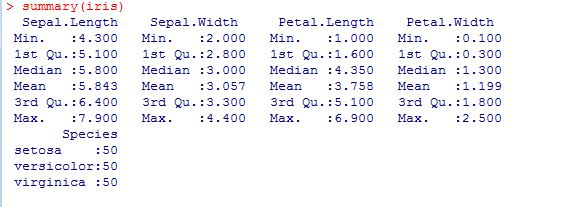
\includegraphics[width=1.2\linewidth]{images/irissummary}
%\caption{}
%\label{fig:irissummary}
\end{figure}
   




%===

{1.12 Working directories}


* You can change your working directly by using the appropriate options on the File menu. 
* To
determine the current working directory, you can use the ``getwd()`` command. 
* To change the
working directory , we would use the ``setwd()`` command.
*  This is quite important as objects
will be imported and exported to and from the specified directory.


%===

\begin{figure}
\centering
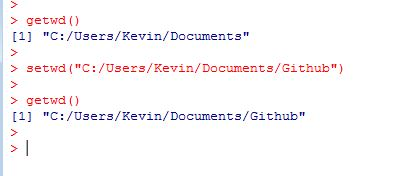
\includegraphics[width=1.2\linewidth]{images/workingdir}

\end{figure}




%===

{1.13 Coming Unstuck}
\Large

*  If you are having trouble with a piece of code that is currently compiling , all you have to do is press ESC, just like many other computing environments.
  

%===

{1.14 Quitting the R environment}
As the front page text indicates, all you have to do to quite the workspace is to type in ``q()``.
You will then be prompted to save your work.

%===

{1.15 Data Objects}
As mentioned previously, R saves data as \textbf{objects}. Examples of data objects are

* Vectors
* Lists
* Dataframes
* Matrices

The simple objects we have created previously are simply single element vectors.

%===

{1.16 Listing all items in a workspace}
To list all items in an R environment, we use the ``ls()`` function. This provides a list of all data
objects accessible. Another useful command is ``objects()``.
\begin{figure}
\centering
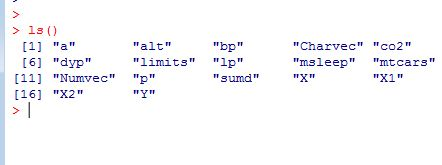
\includegraphics[width=1.2\linewidth]{images/ObjectsList}
%\caption{}
%\label{fig:ObjectsList}
\end{figure}


%===

{1.17 Removing items}

* Sometimes it is desirable to save a subset of your workspace instead of the entire workspace.
* One option is to use the ``rm()`` function to remove unwanted objects right before exiting your R
session; another possibility is to use the ``save()`` function.




 
%===

{1.19 Saving and Loading R Data Objects}
In situations where a good deal of processing must be used on a raw dataset in order to prepare
it for analysis, it may be prudent to save the R objects you create in their internal binary form.
One attractive feature of this scheme is that the objects created can be read by R programs
running on different computer architectures than the one on which they were created, making it
very easy to move your data between different computers. Each time an R session is completed,
you are prompted to save the workspace image, which is a binary file called .RData in the
working directory.

%===

Whenever R encounters such a file in the working directory at the beginning of a session,
it automatically loads it making all your saved objects available again. So one method for

saving your work is to always save your workspace image at the end of an R session. If you
would like to save your workspace image at some other time during your R session, you can use
the save.image() function, which, when called with no arguments, will also save the current
workspace to a file called .RData in the working directory.


% %

{Introduction to R (Continued) }

\item[2.1] Three particularly useful commands    
\item[2.2] Changing GUI options     
\item[2.3] Colours      
\item[2.4] Use of the Semi-Colon Operator     
\item[2.5] The ``apropos()`` Function     
\item[2.6] History       
\item[2.7] The ``sessionInfo()`` Function     
\item[2.8] Time and date functions     
\item[2.9] Logical States      
\item[2.10] Missing Data      
\item[2.11] Files in the Working Directory     



%===

%    2 Introduction to R (Continued)
{2.1 Some particularly useful commands}


The Holy Trinity

* ``help()``
* ``summary()``
* ``help.start()``
* ``apropos()``



%===

{2.2 Changing GUI options}

* We can change the GUI options using the GUI preferences option on the Edit menu.
*  (Important
when teaching R) 
* A demonstration will be done in class.



%===

{2.3 Colours}

* R supported a massive number of colours.
* Type in colours() (or colors()) to see what colours
are supported.




\begin{figure}
\centering
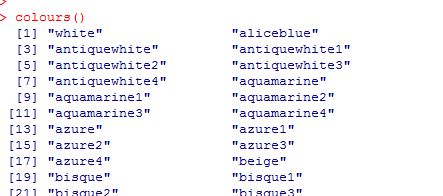
\includegraphics[width=1.2\linewidth]{images/Rcolours}
%\caption{}
%\label{fig:Rcolours}
\end{figure}



%===

{2.4 Use of the Semi-Colon Operator}

* The semi-colon operator at the end of each line of code is not necessary in general, but using it
overcomes errors due to copying and pasting from document soft copies. 
* It is also useful for compacting multiple short statements onto a single line.
* In other programming
languages, such as Octave, using the semicolon in this way has a distinct purpose.


%===

{2.5 The ``apropos()`` Function}

* This function is very useful for determining what functions are available for a particular topic,
although the process requires a great deal of trial and error. 
* Suppose we are looking for a
command to print out the session information. 
* We would use a very short string (e.g. \textbf{essio})
that would plausibly be part of useful function names.



%===

% % SLIDE 1 - COVER SLIDE
\begin{figure}
\centering
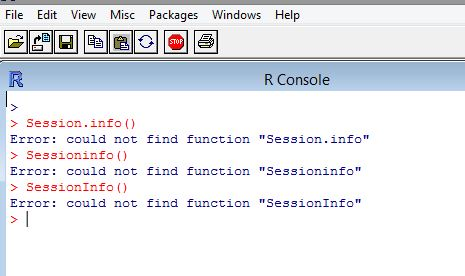
\includegraphics[width=1.2\linewidth]{images/Rapropos1}       
\end{figure}
   
%===

% % SLIDE 1 - COVER SLIDE
\begin{figure}
\centering
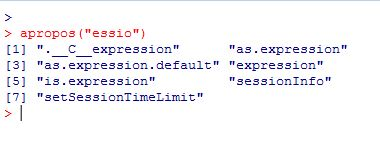
\includegraphics[width=1.2\linewidth]{images/Rapropos2}       
\end{figure}
   
%===

{2.6 History}

* The command ``history()`` is used to obtain the last 25 commands used by ``R}.
* 25 is the default number, you can specify another number.




%===

% % SLIDE 1 - COVER SLIDE
\begin{figure}
\centering
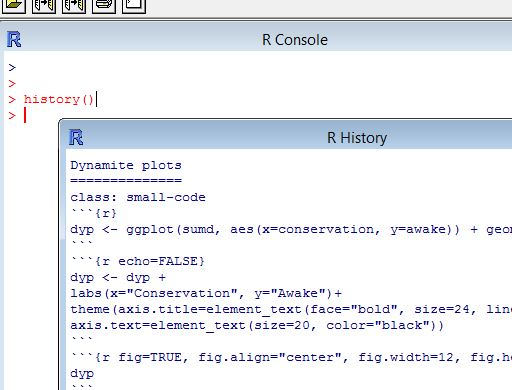
\includegraphics[width=1.2\linewidth]{images/Rhistory}        
\end{figure}
   
%===

{2.7 The ``sessionInfo()`` Function}
To get a description of the version of R and its attached packages used in the current session,
we can use the ``sessionInfo()`` function





{2.7 The ``sessionInfo()`` Function}
\begin{figure}
\centering
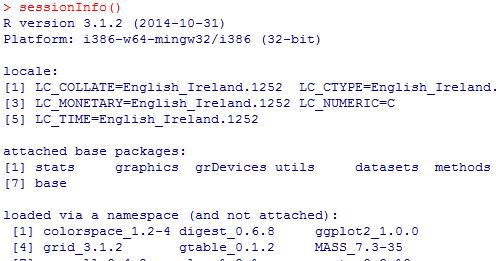
\includegraphics[width=0.99\linewidth]{images/sessionInfo}
%\caption{}
%\label{fig:sessionInfo}
\end{figure}

%===

{2.8 Time and date functions}

* The commands ``Sys.time()`` and ``Sys.Date()`` returns the system’s idea of the current date
with and without time. 
* We can perform some simple algebraic calculations to compute time
differences (i.e. to find out how long some code took to compile).



%===

{System Time}
\begin{figure}
\centering
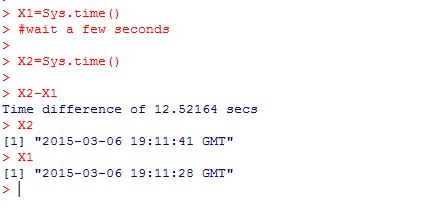
\includegraphics[width=1.2\linewidth]{images/Systime}
%\caption{}
%\label{fig:Systime}
\end{figure}


%===
 
{2.9 Logical States}

* Logical states TRUE and FALSE are simply specified as such, all in capital letters. 
* The
shortcuts T and F are also recognized


%===

{2.10 Missing Data}

* In some cases the entire contents of a vector may not be known. For example, missing data
from a particular data set. * A place can be reserved for this by assigning it the special value
NA.
NA is a logical constant of length 1 which contains a missing value indicator.
*  NA stands
for Not Available.
* Missing values can adversely affect calculations. Add ``na.rm=T} to commands

\begin{framed}
``mean(X,na.rm=T)}
\end{framed}


%===


{2.11 Files in the Working Directory}
It is possibel to call an R script from the working directory, using the ``source()`` function.
\begin{framed}

``source("myfunctions.r")\\
source("mydata.r")}

\end{framed} 
We can also send code put directly to a file in the working directory, using the ``sink()``
command. The first time the command is used, the name of the created file is specified.
Subsequent commands print output directly to this file, until the command is used again to
cease the operation.

%===

\begin{figure}
\centering
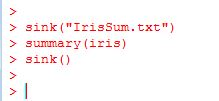
\includegraphics[width=1.2\linewidth]{images/sinkiris}
%\caption{}
%\label{fig:sinkiris}
\end{figure}



%===



\[\mbox{ Section 3 : Inspecting a Data Set } \]

% %

{Section 3 - Inspecting a Data Set }

\item[3.1] Dimensions of a data set 
\item[3.2] The ``summary()`` command   
\item[3.3] Structure of a Data Object 


% % %
%
%{Section 4 : Packages}
%
%  \begin{semiverbatim}
%  4.1 Packages 
%  4.2 Using and Installing packages 
%  4.2.1 Version of R 
%  \end{semiverbatim}
%
% 
%
%\end{document}
% %
%
%{Part 5 - Data Creation, Data Entry, Data Import and Export}
%\begin{framed}
%\begin{semiverbatim}
%5.1 The c() command 
%5.1.1 Vector of Numeric Values
%5.1.2 Vector of Character Values
%5.1.3 Vector of Logical Values 
%5.2 The scan() command 
%5.2.1 Characters with the scan() command
%5.3 Using the data editor
%5.4 Spreadsheet Interface 
%\end{semiverbatim}
%\end{framed}
%
%

%===

{Section 3 Inspecting a Data Set}
 
\textbf{Summary of useful commands}

* ``dim()`` and ``length()``
* ``nrow()`` and ``ncol()``
* ``names()``
* ``summary()``
* ``tail()``
* ``head()``
* ``describe()`` (from the \textbf{psych} package)


%===


{3.1 Dimensions of a data set}

* We have remarked that some data sets are very large. 
* This is perhaps a good place to consider
summary information about data objects. 
* For a simple vector, a useful command to determine
the length (remark: sample size) is the function ``length()``.

\begin{framed}
``Y=4:18}
``length(Y)}

\end{framed}
For more complex data sets ( and data frames which we will see later) , we have several
tools for assessing the size of data.

%===

\begin{figure}
\centering
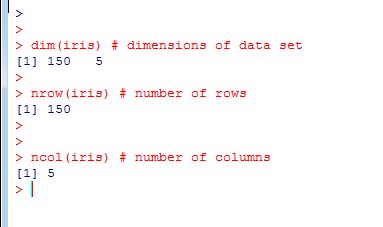
\includegraphics[width=1.2\linewidth]{images/dimsiris}
%\caption{}
%\label{fig:dimsiris}
\end{figure}




%===

{Column (Variable) names and Row names}

* We can also determine the row names and column names using the functions ``rownames()``
and ``colnames()``. 
* If there are no specific row or column names, the command will just return
the indices.

\begin{figure}
\centering
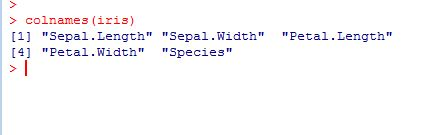
\includegraphics[width=1.0\linewidth]{images/colnamesiris}
%\caption{}
%\label{fig:colnamesiris}
\end{figure}


%===

{3.2 The ``summary()`` command}

* The command ``summary()`` is one of the most useful commands in ``R}. 
* It is a generic function used
to produce result summaries of the results of various functions. 
* The function invokes particular
methods which depend on the class of the first argument. 
* In other words, ``R} picks out the most
suitable type of summary for that data.


%===



\begin{figure}
\centering
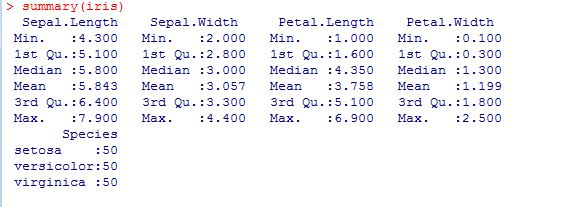
\includegraphics[width=0.99\linewidth]{images/irissummary}

\end{figure}
``summary()`` is particularly useful for manipulating data from more complex data objects.


%===


{3.3 Structure of a Data Object}

The structure, class and storage mode of an object can be determined using the following
commands. Try out a few.

*  ``str()``
*  ``class()``
*  ``mode()``




%===

\begin{figure}
\centering
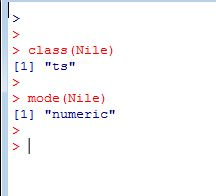
\includegraphics[width=0.7\linewidth]{images/classnile}
%\caption{}
%\label{fig:classnile}
\end{figure}



%===

\begin{figure}
\centering
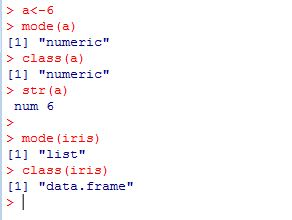
\includegraphics[width=0.9\linewidth]{images/modeclass}

\end{figure}




%===

{Checking and Transforming Types}


* The ``is} family of commands can check if an object is of a certain type.

* The ``as} family of commands can (often) convert an object to a specified type (in some cases not feasible).




%===

{Checking and Transforming Types}
% % SLIDE 1 - COVER SLIDE
\begin{figure}
\centering
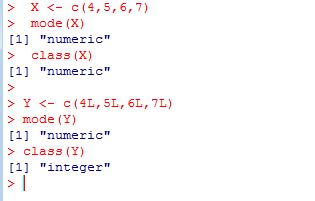
\includegraphics[width=1.2\linewidth]{images/numerictypes}    
\end{figure}
 
%===


{Checking and Transforming Types}
% % SLIDE 1 - COVER SLIDE
\begin{figure}
\centering
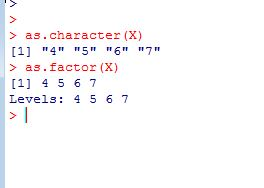
\includegraphics[width=1.2\linewidth]{images/typeconversion} 
\end{figure}
   
%===



\[\mbox{ Section 4 : Packages } \]


{Packages}


* A Package in ``R} is a file containing a collection of objects which have some common purpose.
* Packages enhance the capabilties and scope for research in a certain field. 
* For example, the
package MASS contains objects associated with the Venables and Ripleys ``\textit{Modern Applied
Statistics with S}”. 



%= %



\begin{figure}
\centering
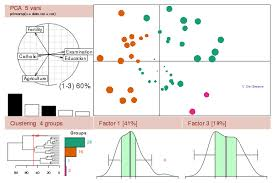
\includegraphics[width=0.97\linewidth]{CRAN}
%\caption{Comprehensive R Archive Network}

\end{figure}





%= %
 
{R Packages}


* ``10 R packages I wish I knew about earlier" - Drew Conway (Yhat.com, February 2013)
 * ``The HadleyVerse" - Hadley Wickham


*  ggplot2, dplyr, reshape, lubridate, stringr

*  With Romain Francois, Dianne Cook and Garret Grolemund.


* Dr Brendan Haplin (UL): lme4 ,TraMineR, Gelman's arm, MASS, foreign. 

* Shiny - Web Applications with ``R}


%= %
 
{R Packages}


* 
Some examples of packages are Actuar, written for actuarial science, and
QRMlib, which complements the Quantitative Risk Management The command library()
lists all the available packages. 

* To load a particular package, for example MASS, we would
write
\begin{framed}
``library(MASS)}
\end{framed}

%= %


{Packages}

* The CRAN package repository features 6107 available packages. 
* Packages contain
various functions and data sets for numerous purposes, e.g.
\textbf{\textit{ggplot2}} package, \textbf{\textit{AER}} package, \textbf{\textit{survival}} package, etc.
* Some packages are part of the basic installation. Others can be
downloaded from CRAN.
* To access all of the functions and data sets in a particular package,
it must be loaded into the workspace. 
* For example, to load the
\textbf{\textit{ggplot2}} package:


\begin{framed}
``install.packages(ggplot2)}

``library(ggplot2)}
\end{framed}

%===

{4.2 Using and Installing packages}

* Many packages come with R. To use them in an R session, you need to load the package, as
previously demonstrated.
* Some packages are not automatically installed when you install R but they need to be downloaded
and installed individually. 
* We must first install them using the install.packages()
function, which typically downloads the package from CRAN and installs it for use. (follow the
instructions as indicated).



%===

{4.2.1 Version of R}
Many packages will require you to have the most recent version of R and also other packages.
It is a good idea to update regularly.

%===

\[\mbox{Section 5 : Data Creation, Data Entry, Data Import and Export}\]

%===

{5.1 The ``c()`` command}
To create a simple data set, known as a vector, we use the c() command to create the vector.
\begin{figure}
\centering
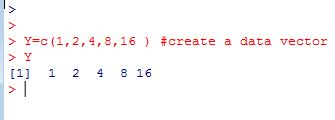
\includegraphics[width=1.2\linewidth]{images/makevector1}
%\caption{}
%\label{fig:makevector1}
\end{figure}



%===

{Vectors}
\begin{figure}
\centering
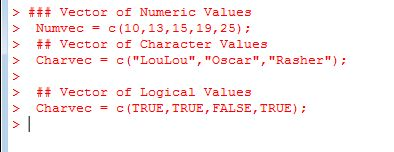
\includegraphics[width=1.2\linewidth]{images/makevectors}
%\caption{}
%\label{fig:makevectors}
\end{figure}


%===

{Vectors} 
Vectors can be bound together either by row or by column.
\begin{figure}
\centering
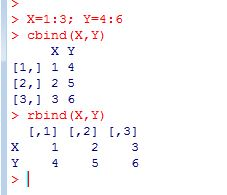
\includegraphics[width=1.0\linewidth]{images/cbindrbind}
\end{figure}


%===

{5.2 The scan() command}

* The ``scan()`` function is a useful method of inputting data quickly. 
* You can use to quickly copy
and paste values into the ``R} environment. It is best used in the manner as described in the
following example. 
* Create a variable ”X” and use the ``scan()`` function to populate it with
values. 
* Type in a value, and then press return. Once you have entered all the values, press
return again to return to normal operation.


%===

\begin{figure}
\centering
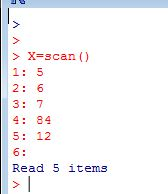
\includegraphics[width=0.8\linewidth]{images/scannumbers}
%\caption{}
%\label{fig:scannumbers}
\end{figure}

Remark: Try the ``edit()`` command on object X.

%===

{5.2.1 Characters with the scan() command}
The scan() command can also be used forinputting character data.
\begin{figure}
\centering
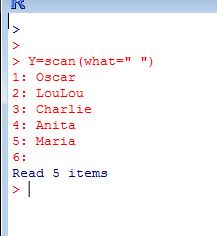
\includegraphics[width=0.7\linewidth]{images/scandognames}
%\caption{}
%\label{fig:scandognames}
\end{figure}


%===

5.3 Using the data editor


%===

{5.4 Spreadsheet Interface}
``R} provides a spreadsheet interface for editing the values of existing data sets. We use the
command ``data.entry()``, and name of the data object as the argument. (Also try out the
fix() command)
%\begin{framed}
%\begin{semiverbatim}
%> data.entry(X) # Edit the data set and exit interface
%> X
%\end{semiverbatim}
%\end{framed}







 \end{document}
